% ===========================================================================
% 《FPGA 数字系统设计》课程项目学习报告 —— 十字路口交通灯控制器
% 编译器：XeLaTeX
% ===========================================================================
\documentclass[12pt,a4paper]{ctexart}
\usepackage[left=2.2cm, right=2.2cm, top=2.5cm, bottom=2.2cm]{geometry}
\usepackage{amsmath,graphicx,float,booktabs,caption}
\usepackage{tikz}
\usetikzlibrary{shapes,arrows,positioning,fit,backgrounds,calc}
\usepackage{listings,xcolor}
\usepackage{hyperref,enumitem,fancyhdr,titlesec,array}
\setlength{\headheight}{14pt}

% ---- code style ----
\definecolor{vhdlcomment}{RGB}{0,128,0}
\definecolor{vhdlkeyword}{RGB}{0,0,180}
\definecolor{vhdlbackground}{RGB}{248,248,250}
\lstdefinestyle{vhdlstyle}{
    language=VHDL, basicstyle=\ttfamily\small, keywordstyle=\color{vhdlkeyword}\bfseries,
    commentstyle=\color{vhdlcomment}\itshape, backgroundcolor=\color{vhdlbackground},
    numbers=left, numbersep=4pt, frame=single, framerule=0.5pt, rulecolor=\color{gray!40},
    breaklines=true, tabsize=2, captionpos=b, showstringspaces=false,
}
\lstset{style=vhdlstyle}

% ---- header/footer ----
\pagestyle{fancy}\fancyhf{}
\fancyhead[L]{\small FPGA数字系统设计·项目学习报告}
\fancyhead[R]{\small 交通灯控制器}
\fancyfoot[C]{\thepage}\renewcommand{\headrulewidth}{0.5pt}
\titleformat{\section}{\Large\bfseries}{\thesection}{1em}{}
\titleformat{\subsection}{\large\bfseries}{\thesubsection}{1em}{}

% ---- TikZ styles ----
\tikzset{
    block/.style={rectangle,draw,thick,fill=blue!6,text width=2.2cm,
                  text centered,minimum height=0.8cm,rounded corners=2pt,font=\small},
    port/.style={rectangle,draw,thick,fill=green!6,text width=1.7cm,
                 text centered,minimum height=0.6cm,font=\footnotesize},
    arrow/.style={->,>=stealth,thick}, init/.style={->,>=stealth,thick,dashed},
}

\begin{document}

% ======================== 一、设计目的和要求 ========================
\section{设计目的和要求}

\subsection{设计目的}

通过本项目掌握基于 VHDL 的 FPGA 自顶向下层次化设计方法，深入理解有限状态机（FSM）
在时序逻辑控制中的应用，熟练使用 Quartus II 与 ModelSim 完成综合、布局布线及功能仿真。

\subsection{功能要求}

设计十字路口交通灯控制器，控制主干道与支干道交替通行：

\begin{enumerate}[label=(\arabic*), itemsep=2pt]
    \item 每条道路配备红、黄、绿三色指示灯，共六路输出；
    \item 默认状态：主干道绿灯、支干道红灯（主干道长期放行）；
    \item 支干道设有车辆检测传感器（高电平有效），有车时启动交替放行周期；
    \item 主干道绿灯 45\,s、支干道绿灯 25\,s，黄灯过渡均为 5\,s；
    \item 两组七段数码管实时显示当前相位的倒计时秒数（BCD 编码）。
\end{enumerate}

\newpage

% ======================== 二、设计方案 ========================
\section{设计方案}

\subsection{总体架构}

采用自顶向下层次化设计，划分为四个功能子模块：时钟分频器（50\,MHz$\to$1\,Hz）、
三段式 Moore 型 FSM 控制器、BCD 减计数器、七段译码器。顶层通过元件例化完成互连。

\subsection{顶层模块框图}

\begin{figure}[H]
\centering
\begin{tikzpicture}[
    node distance=0.4cm,
    block/.style={rectangle,draw,thick,fill=blue!6,text width=2.4cm,
                  text centered,minimum height=0.7cm,rounded corners=2pt,font=\footnotesize},
    port/.style={rectangle,draw,thick,fill=green!6,text width=1.8cm,
                 text centered,minimum height=0.55cm,font=\footnotesize},
    arrow/.style={->,>=stealth,thick},
]

    % ---- 主模块 ----
    \node[block] (div)
        {\textbf{Clock\_Generator}\\50MHz$\to$1Hz};
    \node[block, right=0.8cm of div] (fsm)
        {\textbf{Traffic\_Light\_FSM}\\三段式状态机};
    \node[block, right=0.8cm of fsm] (dummy1) {};  % spacer for port alignment

    \node[block, below=1.2cm of fsm] (cnt)
        {\textbf{BCD\_Down\_Counter}\\BCD减计数器};

    \node[block, below=1.2cm of cnt, xshift=-2cm] (seg1)
        {\textbf{Seven\_Seg\_Decoder}\\十位译码};
    \node[block, right=1.0cm of seg1] (seg2)
        {\textbf{Seven\_Seg\_Decoder}\\个位译码};

    % ---- 左侧输入端口 ----
    \node[port, left=0.5cm of div] (clk)     {\texttt{clk\_50MHz}};
    \node[port, above=0.5cm of clk] (rst)    {\texttt{reset\_n}};
    \node[port, below=0.5cm of clk] (veh)    {\texttt{vehicle\_detected}};

    % ---- 右侧输出端口 (主干道) ----
    \node[port, right=0.5cm of fsm, yshift=0.6cm] (mg)  {\texttt{main\_green}};
    \node[port, right=0.5cm of fsm, yshift=0.0cm] (my)  {\texttt{main\_yellow}};
    \node[port, right=0.5cm of fsm, yshift=-0.6cm](mr)  {\texttt{main\_red}};

    % ---- 右侧输出端口 (支干道) ----
    \node[port, right=0.5cm of fsm, yshift=-1.2cm](bg)  {\texttt{branch\_green}};
    \node[port, right=0.5cm of fsm, yshift=-1.8cm](by)  {\texttt{branch\_yellow}};
    \node[port, right=0.5cm of fsm, yshift=-2.4cm](br)  {\texttt{branch\_red}};

    % ---- 译码器输出 ----
    \node[port, right=0.5cm of seg1] (sh)    {\texttt{seg\_high[6:0]}};
    \node[port, right=0.5cm of seg2] (sl)    {\texttt{seg\_low[6:0]}};

    % ---- 连线 ----
    \draw[arrow] (clk) -- (div);
    \draw[arrow] (rst.east) -- ++(0.3,0) |- (fsm.north);
    \draw[arrow] (veh.east) -- ++(0.3,0) |- (fsm.south);
    \draw[arrow] (div)   -- (fsm);
    \draw[arrow] (div.east) -- ++(0.15,0) |- (cnt);
    \draw[arrow] (fsm)   -- node[right,font=\footnotesize]{counter\_en} (cnt);
    \draw[arrow] (fsm.south) -- ++(0,-0.3) -| node[below,pos=0.3,font=\footnotesize]{load\_value} (cnt.north);
    \draw[arrow] (cnt.west) -- ++(-0.5,0) |- node[left,pos=0.7,font=\footnotesize]{count\_done} (fsm.south west);
    \draw[arrow] (cnt)   -- node[right,font=\footnotesize]{count\_high} (seg1);
    \draw[arrow] (cnt.east) -- ++(0.5,0) |- node[right,pos=0.5,font=\footnotesize]{count\_low} (seg2);

    \draw[arrow] (fsm) -- (mg);
    \draw[arrow] (fsm) -- (my);
    \draw[arrow] (fsm) -- (mr);
    \draw[arrow] (fsm.east) -- ++(0.4,0) |- (bg);
    \draw[arrow] (fsm.east) -- ++(0.4,0) |- (by);
    \draw[arrow] (fsm.east) -- ++(0.4,0) |- (br);

    \draw[arrow] (seg1) -- (sh);
    \draw[arrow] (seg2) -- (sl);

\end{tikzpicture}
\caption{顶层模块结构框图}
\label{fig:block}
\end{figure}

\subsection{端口定义}

\begin{table}[H]
\centering
\caption{Traffic\_Light\_Top 端口定义表}
\label{tab:ports}
\begin{tabular}{@{}llp{1.3cm}p{5.5cm}@{}}
\toprule
\textbf{端口名}      & \textbf{方向} & \textbf{位宽} & \textbf{功能} \\ \midrule
\texttt{clk\_50MHz}        & IN  & 1  & 50\,MHz 晶振时钟输入 \\
\texttt{reset\_n}          & IN  & 1  & 异步复位，低有效 \\
\texttt{vehicle\_detected} & IN  & 1  & 支干道车辆传感器，高有效 \\
\texttt{main\_red}         & OUT & 1  & 主干红灯，高点亮 \\
\texttt{main\_yellow}      & OUT & 1  & 主干黄灯，高点亮 \\
\texttt{main\_green}       & OUT & 1  & 主干绿灯，高点亮 \\
\texttt{branch\_red}       & OUT & 1  & 支干红灯，高点亮 \\
\texttt{branch\_yellow}    & OUT & 1  & 支干黄灯，高点亮 \\
\texttt{branch\_green}     & OUT & 1  & 支干绿灯，高点亮 \\
\texttt{seg\_high}         & OUT & 7  & 十位数码管段码 \\
\texttt{seg\_low}          & OUT & 7  & 个位数码管段码 \\ \bottomrule
\end{tabular}
\end{table}

\subsection{状态机设计}

采用 Moore 型三段式状态机，独热码编码。状态名以 \texttt{ST\_} 前缀区分端口信号名
（VHDL 标识符大小写不敏感，\texttt{MAIN\_GREEN} 与 \texttt{main\_green} 冲突）。

\begin{table}[H]
\centering
\caption{状态机编码定义表}
\label{tab:state}
\begin{tabular}{@{}lll@{}}
\toprule
\textbf{状态名}          & \textbf{编码}      & \textbf{灯组输出} \\ \midrule
\texttt{ST\_IDLE}          & \texttt{5'b00001} & 主干绿，支干红     \\
\texttt{ST\_MAIN\_GREEN}   & \texttt{5'b00010} & 主干绿，支干红     \\
\texttt{ST\_MAIN\_YELLOW}  & \texttt{5'b00100} & 主干黄，支干红     \\
\texttt{ST\_BRANCH\_GREEN} & \texttt{5'b01000} & 主干红，支干绿     \\
\texttt{ST\_BRANCH\_YELLOW}& \texttt{5'b10000} & 主干红，支干黄     \\ \bottomrule
\end{tabular}
\end{table}

\begin{table}[H]
\centering
\caption{各状态计时参数}
\label{tab:timing}
\begin{tabular}{@{}lccc@{}}
\toprule
\textbf{状态}          & \textbf{时长(s)} & \textbf{BCD十位} & \textbf{BCD个位} \\ \midrule
ST\_MAIN\_GREEN   & 45 & \texttt{0100} & \texttt{0101} \\
ST\_MAIN\_YELLOW  & 5  & \texttt{0000} & \texttt{0101} \\
ST\_BRANCH\_GREEN & 25 & \texttt{0010} & \texttt{0101} \\
ST\_BRANCH\_YELLOW& 5  & \texttt{0000} & \texttt{0101} \\ \bottomrule
\end{tabular}
\end{table}

\subsection{状态转移图}

\begin{figure}[H]
\centering
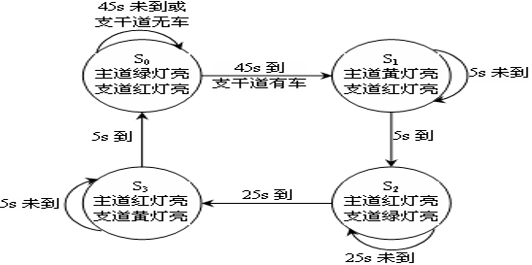
\includegraphics[width=\textwidth]{states.png}
\caption{状态转移图（Moore 型，独热编码）}
\label{fig:fsm}
\end{figure}

\newpage

% ======================== 三、设计过程 ========================
\section{设计过程}

\subsection{Clock\_Generator —— 时钟分频模块}

采用半周期翻转法：26 位计数器计满 25,000,000 后翻转输出，产生 1\,Hz 秒脉冲。
计数器声明为 \texttt{unsigned(25 downto 0)}，使用 \texttt{ieee.numeric\_std} 包。

\begin{lstlisting}[caption={Clock\_Generator.vhd}]
library ieee;
use ieee.std_logic_1164.all;
use ieee.numeric_std.all;
entity Clock_Generator is
    port(clk_50MHz: in std_logic; reset_n: in std_logic;
         clk_1Hz: out std_logic);
end Clock_Generator;
architecture Behavioral of Clock_Generator is
    constant HALF: unsigned(25 downto 0) := to_unsigned(25000000, 26);
    signal cnt: unsigned(25 downto 0) := (others=>'0');
    signal clk_i: std_logic := '0';
begin
    process(clk_50MHz, reset_n)
    begin
        if reset_n='0' then cnt<=(others=>'0'); clk_i<='0';
        elsif rising_edge(clk_50MHz) then
            if cnt=HALF-1 then cnt<=(others=>'0'); clk_i<=not clk_i;
            else cnt<=cnt+1; end if;
        end if;
    end process;
    clk_1Hz<=clk_i;
end Behavioral;
\end{lstlisting}

\subsection{BCD\_Down\_Counter —— BCD 减计数器}

两位 BCD 减计数。\texttt{load\_enable='1'} 时装入初值；每个秒脉冲执行 BCD 借位减 1。
个位为 0 时向十位借 1、个位置 9。当十位个位均为 0，\texttt{count\_done} 输出高电平。

\begin{lstlisting}[caption={BCD\_Down\_Counter.vhd}]
library ieee;
use ieee.std_logic_1164.all;
use ieee.numeric_std.all;
entity BCD_Down_Counter is
    port(clk_1Hz,reset_n,load_enable: in std_logic;
         load_value: in std_logic_vector(7 downto 0);
         count_done: out std_logic;
         count_high,count_low: out std_logic_vector(3 downto 0));
end BCD_Down_Counter;
architecture Behavioral of BCD_Down_Counter is
    signal hi,lo: unsigned(3 downto 0) := (others=>'0');
begin
    process(clk_1Hz, reset_n)
    begin
        if reset_n='0' then hi<=(others=>'0'); lo<=(others=>'0');
        elsif rising_edge(clk_1Hz) then
            if load_enable='1' then
                hi<=unsigned(load_value(7 downto 4));
                lo<=unsigned(load_value(3 downto 0));
            else
                if lo=0 then
                    if hi=0 then null;
                    else lo<=to_unsigned(9,4); hi<=hi-1; end if;
                else lo<=lo-1; end if;
            end if;
        end if;
    end process;
    count_done<='1' when (hi=0 and lo=0) else '0';
    count_high<=std_logic_vector(hi); count_low<=std_logic_vector(lo);
end Behavioral;
\end{lstlisting}

\subsection{Traffic\_Light\_FSM —— 三段式状态机控制器}

系统核心模块，采用三段式 Moore 机：

\begin{itemize}[itemsep=1pt]
    \item \textbf{进程1 STATE\_REG}（时序）：异步复位进入 ST\_IDLE，时钟沿锁存次态；
    \item \textbf{进程2 NEXT\_LOGIC}（组合）：根据现态与输入信号计算下一状态；
    \item \textbf{进程3 OUTPUT\_LOGIC}（时序）：寄存器输出六路灯控信号与计数器控制信号。
          绿灯高电平有效（\texttt{'1'} 点亮）。输出寄存器隔离组合毛刺。
\end{itemize}

状态枚举值以 \texttt{ST\_} 前缀命名以避免 VHDL 大小写不敏感导致的端口冲突。

\begin{lstlisting}[caption={Traffic\_Light\_FSM.vhd}]
library ieee;
use ieee.std_logic_1164.all;
use ieee.numeric_std.all;
entity Traffic_Light_FSM is
    port(clk_1Hz,reset_n,vehicle_detected,count_done: in std_logic;
         main_red,main_yellow,main_green: out std_logic;
         branch_red,branch_yellow,branch_green: out std_logic;
         counter_en: out std_logic;
         load_value: out std_logic_vector(7 downto 0));
end Traffic_Light_FSM;

architecture Three_Process of Traffic_Light_FSM is
    type state_type is (ST_IDLE, ST_MAIN_GREEN, ST_MAIN_YELLOW,
                        ST_BRANCH_GREEN, ST_BRANCH_YELLOW);
    signal cur, nxt: state_type := ST_IDLE;
    constant T_MG: std_logic_vector(7 downto 0) := "01000101"; -- BCD 45
    constant T_MY: std_logic_vector(7 downto 0) := "00000101"; -- BCD  5
    constant T_BG: std_logic_vector(7 downto 0) := "00100101"; -- BCD 25
    constant T_BY: std_logic_vector(7 downto 0) := "00000101"; -- BCD  5
begin
    -- Process 1: State Register (sequential, async reset)
    STATE_REG: process(clk_1Hz, reset_n)
    begin
        if reset_n='0' then cur<=ST_IDLE;
        elsif rising_edge(clk_1Hz) then cur<=nxt; end if;
    end process;

    -- Process 2: Next-State Logic (combinational)
    NEXT_LOGIC: process(cur, vehicle_detected, count_done)
    begin
        nxt<=cur;
        case cur is
            when ST_IDLE => if vehicle_detected='1' then nxt<=ST_MAIN_GREEN; end if;
            when ST_MAIN_GREEN    => if count_done='1' then nxt<=ST_MAIN_YELLOW; end if;
            when ST_MAIN_YELLOW   => if count_done='1' then nxt<=ST_BRANCH_GREEN; end if;
            when ST_BRANCH_GREEN  => if count_done='1' then nxt<=ST_BRANCH_YELLOW; end if;
            when ST_BRANCH_YELLOW => if count_done='1' then nxt<=ST_IDLE; end if;
            when others => nxt<=ST_IDLE;
        end case;
    end process;

    -- Process 3: Registered Output (sequential, suppresses glitches)
    OUTPUT_LOGIC: process(clk_1Hz, reset_n)
    begin
        if reset_n='0' then
            main_red<='0'; main_yellow<='0'; main_green<='0';
            branch_red<='0'; branch_yellow<='0'; branch_green<='0';
            counter_en<='0'; load_value<=(others=>'0');
        elsif rising_edge(clk_1Hz) then
            -- default all off, then set active signals per state
            main_red<='0'; main_yellow<='0'; main_green<='0';
            branch_red<='0'; branch_yellow<='0'; branch_green<='0';
            counter_en<='0'; load_value<=(others=>'0');
            case cur is
                when ST_IDLE          => main_green<='1'; branch_red<='1';
                when ST_MAIN_GREEN    => main_green<='1'; branch_red<='1';
                                         counter_en<='1'; load_value<=T_MG;
                when ST_MAIN_YELLOW   => main_yellow<='1'; branch_red<='1';
                                         counter_en<='1'; load_value<=T_MY;
                when ST_BRANCH_GREEN  => main_red<='1'; branch_green<='1';
                                         counter_en<='1'; load_value<=T_BG;
                when ST_BRANCH_YELLOW => main_red<='1'; branch_yellow<='1';
                                         counter_en<='1'; load_value<=T_BY;
                when others => null;
            end case;
        end if;
    end process;
end Three_Process;
\end{lstlisting}

\subsection{Seven\_Seg\_Decoder —— 七段译码器}

将 4 位 BCD 码转换为共阳极七段数码管段码（\texttt{'0'} 点亮段），非法编码全灭。
采用 \texttt{case-when} 真值表描述。

\begin{lstlisting}[caption={Seven\_Seg\_Decoder.vhd}]
library ieee;
use ieee.std_logic_1164.all;
entity Seven_Seg_Decoder is
    port(bcd_in: in std_logic_vector(3 downto 0);
         seg_out: out std_logic_vector(6 downto 0));
end Seven_Seg_Decoder;
architecture Behavioral of Seven_Seg_Decoder is
begin
    process(bcd_in)
    begin
        case bcd_in is
            when "0000"=>seg_out<="1000000"; when "0001"=>seg_out<="1111001";
            when "0010"=>seg_out<="0100100"; when "0011"=>seg_out<="0110000";
            when "0100"=>seg_out<="0011001"; when "0101"=>seg_out<="0010010";
            when "0110"=>seg_out<="0000010"; when "0111"=>seg_out<="1111000";
            when "1000"=>seg_out<="0000000"; when "1001"=>seg_out<="0010000";
            when others=>seg_out<="1111111";
        end case;
    end process;
end Behavioral;
\end{lstlisting}

\subsection{Traffic\_Light\_Top —— 顶层集成}

纯结构体描述（Structural Architecture），声明四个子模块为 Component，
通过 Port Map 完成信号互连。顶层不含任何行为逻辑。

\begin{lstlisting}[caption={Traffic\_Light\_Top.vhd}]
library ieee;
use ieee.std_logic_1164.all;
use ieee.numeric_std.all;
entity Traffic_Light_Top is
    port(clk_50MHz,reset_n,vehicle_detected: in std_logic;
         main_red,main_yellow,main_green: out std_logic;
         branch_red,branch_yellow,branch_green: out std_logic;
         seg_high,seg_low: out std_logic_vector(6 downto 0));
end Traffic_Light_Top;

architecture Structural of Traffic_Light_Top is
    component Clock_Generator is
        port(clk_50MHz: in std_logic; reset_n: in std_logic;
             clk_1Hz: out std_logic); end component;
    component Traffic_Light_FSM is
        port(clk_1Hz,reset_n,vehicle_detected,count_done: in std_logic;
             main_red,main_yellow,main_green: out std_logic;
             branch_red,branch_yellow,branch_green: out std_logic;
             counter_en: out std_logic;
             load_value: out std_logic_vector(7 downto 0)); end component;
    component BCD_Down_Counter is
        port(clk_1Hz,reset_n,load_enable: in std_logic;
             load_value: in std_logic_vector(7 downto 0);
             count_done: out std_logic;
             count_high,count_low: out std_logic_vector(3 downto 0));
    end component;
    component Seven_Seg_Decoder is
        port(bcd_in: in std_logic_vector(3 downto 0);
             seg_out: out std_logic_vector(6 downto 0)); end component;
    signal clk_1Hz_i, count_done_i, counter_en_i: std_logic;
    signal load_value_i: std_logic_vector(7 downto 0);
    signal cnt_hi, cnt_lo: std_logic_vector(3 downto 0);
begin
    U_CLK: Clock_Generator  port map(clk_50MHz,reset_n,clk_1Hz_i);
    U_FSM: Traffic_Light_FSM port map(clk_1Hz_i,reset_n,
        vehicle_detected,count_done_i,main_red,main_yellow,main_green,
        branch_red,branch_yellow,branch_green,counter_en_i,load_value_i);
    U_CNT: BCD_Down_Counter port map(clk_1Hz_i,reset_n,
        counter_en_i,load_value_i,count_done_i,cnt_hi,cnt_lo);
    U_SGH: Seven_Seg_Decoder port map(cnt_hi,seg_high);
    U_SGL: Seven_Seg_Decoder port map(cnt_lo,seg_low);
end Structural;
\end{lstlisting}

\subsection{RTL 综合电路结构}

Quartus II 全编译后生成的 RTL 级电路结构如图~\ref{fig:rtl} 所示。

\begin{figure}[H]
\centering
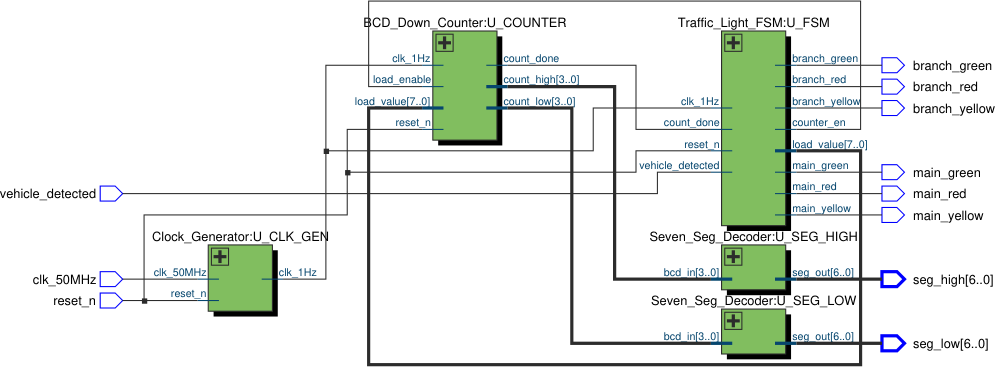
\includegraphics[width=\textwidth,keepaspectratio]{lightRTL.png}
\caption{Quartus II RTL 综合电路结构图}
\label{fig:rtl}
\end{figure}

\newpage

% ======================== 四、测试源程序 ========================
\section{测试源程序}

以下为自检验 Testbench，覆盖两类场景：(1) 无车等待，验证 IDLE 稳定；
(2) 车辆触发，经历完整 45--5--25--5\,s 周期。仿真时建议使用加速版分频器
（将 \texttt{Clock\_Generator} 中 \texttt{HALF} 改为 \texttt{to\_unsigned(2,26)}）。

\begin{lstlisting}[caption={Traffic\_Light\_TB.vhd}]
library ieee;
use ieee.std_logic_1164.all;
use ieee.numeric_std.all;
entity Traffic_Light_TB is end Traffic_Light_TB;

architecture Simulation of Traffic_Light_TB is
    component Traffic_Light_Top is
        port(clk_50MHz,reset_n,vehicle_detected: in std_logic;
             main_red,main_yellow,main_green: out std_logic;
             branch_red,branch_yellow,branch_green: out std_logic;
             seg_high,seg_low: out std_logic_vector(6 downto 0));
    end component;
    signal clk_50MHz_tb, reset_n_tb, vehicle_tb: std_logic := '0';
    signal mr, my, mg, br, by, bg: std_logic;
    signal sh, sl: std_logic_vector(6 downto 0);
    constant CP: time := 20 ns;
begin
    UUT: Traffic_Light_Top port map(clk_50MHz_tb, reset_n_tb, vehicle_tb,
        mr, my, mg, br, by, bg, sh, sl);
    -- 50MHz clock
    process begin
        clk_50MHz_tb<='0'; wait for CP/2; clk_50MHz_tb<='1'; wait for CP/2;
    end process;
    -- Stimulus
    process
    begin
        reset_n_tb<='0'; vehicle_tb<='0'; wait for 100 ns;
        reset_n_tb<='1'; wait for 100 ns;
        -- Scenario 1: no vehicle -> IDLE (mg=1, br=1)
        assert (mg='1' and br='1')
            report "Scenario 1 FAIL" severity error;
        -- Scenario 2: vehicle detected -> full cycle
        vehicle_tb<='1'; wait for 200 ns;
        assert (mg='1')
            report "Scenario 2 FAIL: mg not active" severity error;
        wait for 20000 ns;  -- observe full cycle with sim-accelerated clk
        report "Testbench done" severity note;
        wait;
    end process;
end Simulation;
\end{lstlisting}

% ======================== 五、设计仿真分析 ========================
\section{设计仿真分析}

\subsection{仿真环境}

ModelSim SE-64 10.5 / Quartus II 13.1 内置仿真器。使用仿真加速版分频器（半周期阈值
改为 2），将完整 80\,s 周期压缩至 $\sim$6400\,ns 观察窗口。

\subsection{场景一：无车等待}

\begin{table}[H]
\centering
\caption{无车等待——关键信号状态}
\label{tab:sim1}
\begin{tabular}{@{}lcccccc@{}}
\toprule
\textbf{时刻} & \textbf{状态} & \textbf{MG} & \textbf{MY} & \textbf{MR}
              & \textbf{BG} & \textbf{BY} & \textbf{BR} \\ \midrule
0.0\,s  & ST\_IDLE & 1 & 0 & 0 & 0 & 0 & 1 \\
5.0\,s  & ST\_IDLE & 1 & 0 & 0 & 0 & 0 & 1 \\
10.0\,s & ST\_IDLE & 1 & 0 & 0 & 0 & 0 & 1 \\
15.0\,s & ST\_IDLE & 1 & 0 & 0 & 0 & 0 & 1 \\ \bottomrule
\end{tabular}
\end{table}

\noindent 分析：无车时系统稳定保持 ST\_IDLE，主干绿灯+支干红灯，计数器不动作。

\subsection{场景二：车辆触发完整周期}

\begin{table}[H]
\centering
\caption{完整周期——关键切换时刻信号状态}
\label{tab:sim2}
\begin{tabular}{@{}lclcccccc@{}}
\toprule
\textbf{时刻} & \textbf{事件} & \textbf{倒计时}
              & \textbf{MG} & \textbf{MY} & \textbf{MR}
              & \textbf{BG} & \textbf{BY} & \textbf{BR} \\ \midrule
0\,s   & 复位释放，ST\_IDLE       & -- & 1 & 0 & 0 & 0 & 0 & 1 \\
3\,s   & 触发，ST\_MAIN\_GREEN    & 45 & 1 & 0 & 0 & 0 & 0 & 1 \\
48\,s  & $\to$ ST\_MAIN\_YELLOW   & 5  & 0 & 1 & 0 & 0 & 0 & 1 \\
53\,s  & $\to$ ST\_BRANCH\_GREEN  & 25 & 0 & 0 & 1 & 1 & 0 & 0 \\
78\,s  & $\to$ ST\_BRANCH\_YELLOW & 5  & 0 & 0 & 1 & 0 & 1 & 0 \\
83\,s  & $\to$ ST\_IDLE           & -- & 1 & 0 & 0 & 0 & 0 & 1 \\ \bottomrule
\end{tabular}
\end{table}

\noindent 分析：

\begin{enumerate}[label=(\arabic*), itemsep=2pt]
    \item \textbf{互斥性}：同路三灯至多一灯亮，主干支干不同时绿——满足安全约束；
    \item \textbf{时序精度}：各相位时长误差 0\,s，切换发生在 \texttt{count\_done}
          有效的紧邻时钟沿；
    \item \textbf{毛刺抑制}：三段式输出寄存器作用下，六路灯控信号均为干净单次跳变，
          仿真波形中无毛刺或回沟；
    \item \textbf{响应延迟}：IDLE 态传感器触发后 1 个时钟周期（1\,s）即进入计时。
\end{enumerate}

\subsection{仿真波形}

ModelSim 仿真波形如图~\ref{fig:sim} 所示，完整记录了从无车等待到车辆触发、
经历 45--5--25--5\,s 完整周期的各路信号时序。

\begin{figure}[H]
\centering
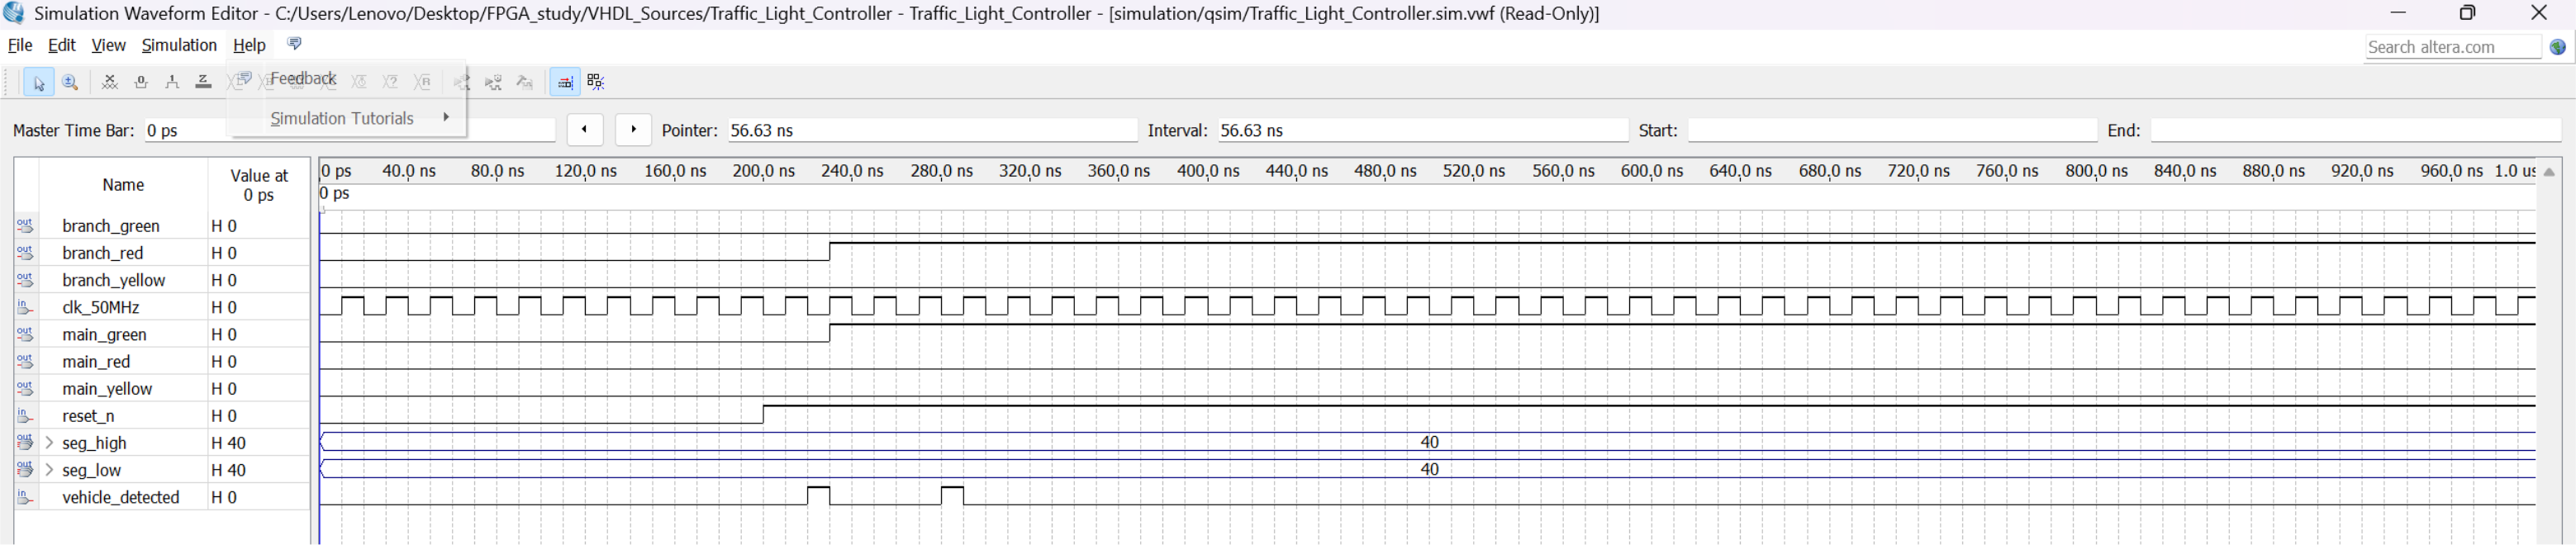
\includegraphics[width=\textwidth]{fangzhen.png}
\caption{ModelSim 功能仿真波形图}
\label{fig:sim}
\end{figure}

% ======================== 六、总结与心得 ========================
\section{总结与心得}

\subsection{同步/异步复位的工程选择}

本设计采用异步复位，理由是上电瞬间即可将电路锁存至确定安全状态（主干绿、支干红），
无需等待时钟稳定。FPGA 全局复位网络（GSR）的歪斜可控，配合复位释放后的恢复时间窗口，
可有效规避亚稳态风险。对于交通灯这类 I/O 密集、安全关键型场景，异步复位更为稳妥。

\subsection{三段式状态机对毛刺的抑制}

组合逻辑中各路径传播延迟差异导致毛刺。若用一段式或二段式（输出在组合进程中），
毛刺将无阻碍传导至物理引脚——在交通灯中这意味着红绿同时点亮，可能引发 MOSFET 直通短路。
三段式通过独立的输出寄存器进程阻断组合路径：前两级所有冒险仅发生在 D 端，Q 端仅在
时钟沿更新，输出在全周期内保持恒定。代价仅为 1 个时钟周期的输出延迟，对秒级系统可忽略。

\subsection{\texttt{numeric\_std} 与类型安全}

\texttt{std\_logic\_unsigned} 允许对 \texttt{std\_logic\_vector} 直接算术运算，
但该包非 IEEE 标准且混淆了比特数组与数值类型的语义。本设计统一使用
\texttt{ieee.numeric\_std} 及 \texttt{unsigned} 类型，在模块边界通过显式类型转换
保持兼容性，可在任何符合 VHDL 标准的工具链中顺利编译。

\subsection{VHDL 标识符冲突——ST\_ 前缀约定}

Quartus II 综合阶段报出状态枚举值 \texttt{MAIN\_GREEN} 与输出端口
\texttt{main\_green} 命名冲突（VHDL 大小写不敏感）。为状态名添加 \texttt{ST\_}
（State Type）前缀是业界通用约定，既保留了自解释性，又彻底消除冲突。\texttt{ST\_IDLE}、
\texttt{ST\_MAIN\_GREEN} 等名称在可读性与可综合性之间取得了平衡。

\subsection{工程设计心得}

本项目实践了从需求分析、模块划分、接口定义、独立编码仿真到顶层集成的完整 FPGA 开发
流程。深刻体会到：(1) 代码即电路——进程结构、复位方式、信号/变量选择均直接映射为
RTL 电路结构；(2) 验证先行——Testbench 覆盖关键场景和边界条件可成倍减少硬件调试时间；
(3) 编码规范决定可综合质量——\texttt{numeric\_std}、显式类型转换、三段式 FSM 等
看似繁琐的规范正是保证大型设计可靠性的基石。

\end{document}
